\noindent In the previous section, we introduced one of the substitution rules considered in this work. In what follows, we first present the remaining two substitution rules and the resulting tilings with rotational symmetry. We then describe the Kannan–Soroker–Kenyon (KSK) criterion~\cite{KanSor92, Ken93}, which is used to obtain the dissections that give rise to these substitution rules. We note that substitution rules were not derived through a systematic, step-by-step procedure; rather, they arose from brute-force exploration guided by the KSK criterion and by techniques for enforcing the \(n\)-fold rotational symmetry property. The latter, which constitutes a different line of investigation, follows a distinct approach that is too lengthy to include here and is currently being studied for a general class of tilings in~\cite{SayDe}.  

Our focus here is therefore on describing the resulting constructions and their properties, rather than providing a procedural method for their derivation.


\subsection{The Substitution Rules and Tilings with \(n-\)Fold Rotational Symmetry}
\noindent Recall that the substitution factor for \(n=13\) is  \(\mu_{13} = \frac{\sin\left(\frac{6\pi}{13}\right)}{\sin\left(\frac{\pi}{13}\right)} \approx 4.148,\) which is equal to the length of the longest diagonal of a regular \(13\)-gon with unit side length. In general, the length of the longest diagonal of a regular \(n\)-gon with unit side length is given by  

\begin{equation}
\mu_n = \frac{\sin\left( \frac{(n-1)\pi}{2n} \right)}{\sin\left( \frac{\pi}{n} \right)}, 
\label{eq:subfac}
\end{equation}  
%%Use \(\) 
\noindent and we use \(\mu_{17}\) and \(\mu_{21}\) as substitution factors for the cases \(n = 17\) and \(n = 21\), respectively. As mentioned in the introduction, this formula first appeared in \cite{NisDanz96} and has since been used to produce several tilings.

The prototiles are $T_{n,1}, T_{n,2}, \dots, T_{n,(n-1)/2}$, where $T_{n,k}$ is an isosceles triangle with legs of length $1$ and opening angle $(n-2k)\pi/n$. By straightforward calculation, the length of the base of $T_{n,k}$ is
\[
s_{n,k} = 2 \sin\left( \frac{(n-2k)\pi}{2n} \right).
\]

For each $n \in \{13,17,21\}$, we denote the corresponding substitution rule by $\sigma_n$. The case $n = 13$ is already shown in Fig.~\ref{fig:13-fold}, while the substitution rules $\sigma_{17}$ and $\sigma_{21}$ are illustrated in the following figures. As in the case $n = 13$, the tiles are equipped with markings, since the dissections corresponding to the substitution rules break the symmetry of the inflated prototiles, and so markings are necessary to indicate the orientations of the tiles. Moreover, each prototile appears in every 1-order supertile, and so $\sigma_{n}$ is primitive.  

\begin{figure}[H]
\center
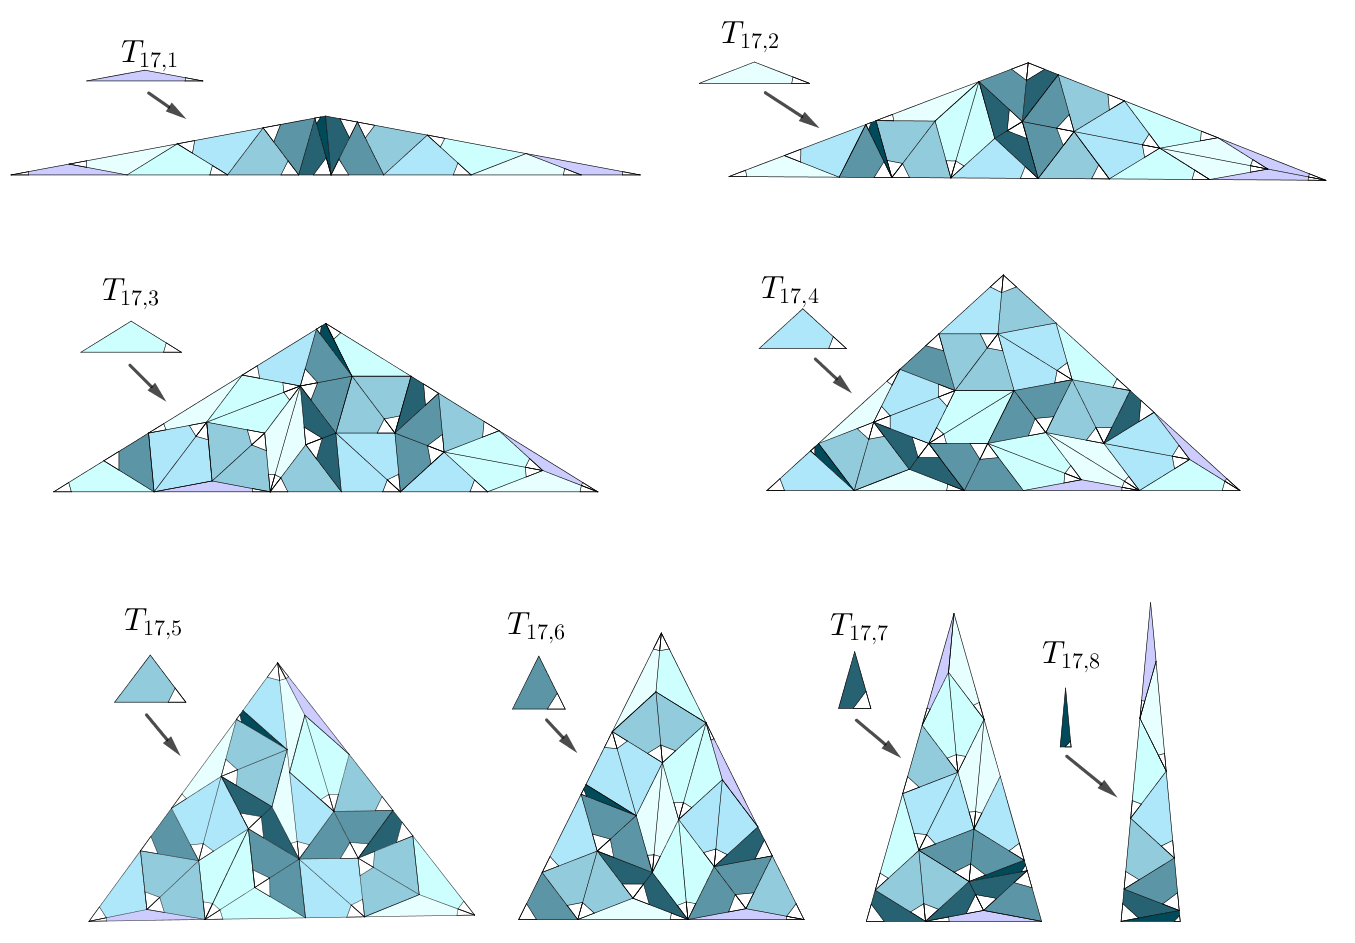
\includegraphics[width=.75\textwidth]{ILCFig4_17-fold}
\caption{The substitution $\sigma_{17}$.  
\label{fig:17-fold}}
\end{figure}

\begin{figure}[H]
\center
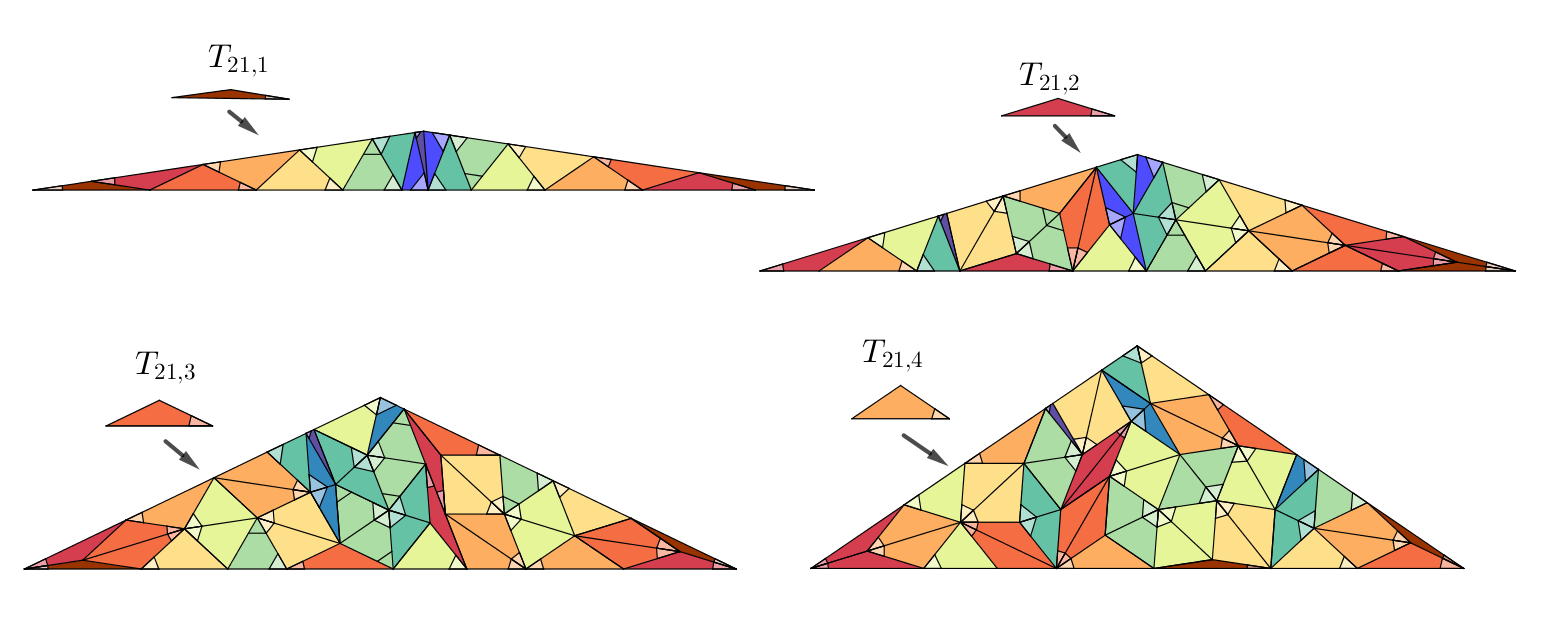
\includegraphics[width=.75\textwidth]{ILCFig5_21-fold_a_}\\
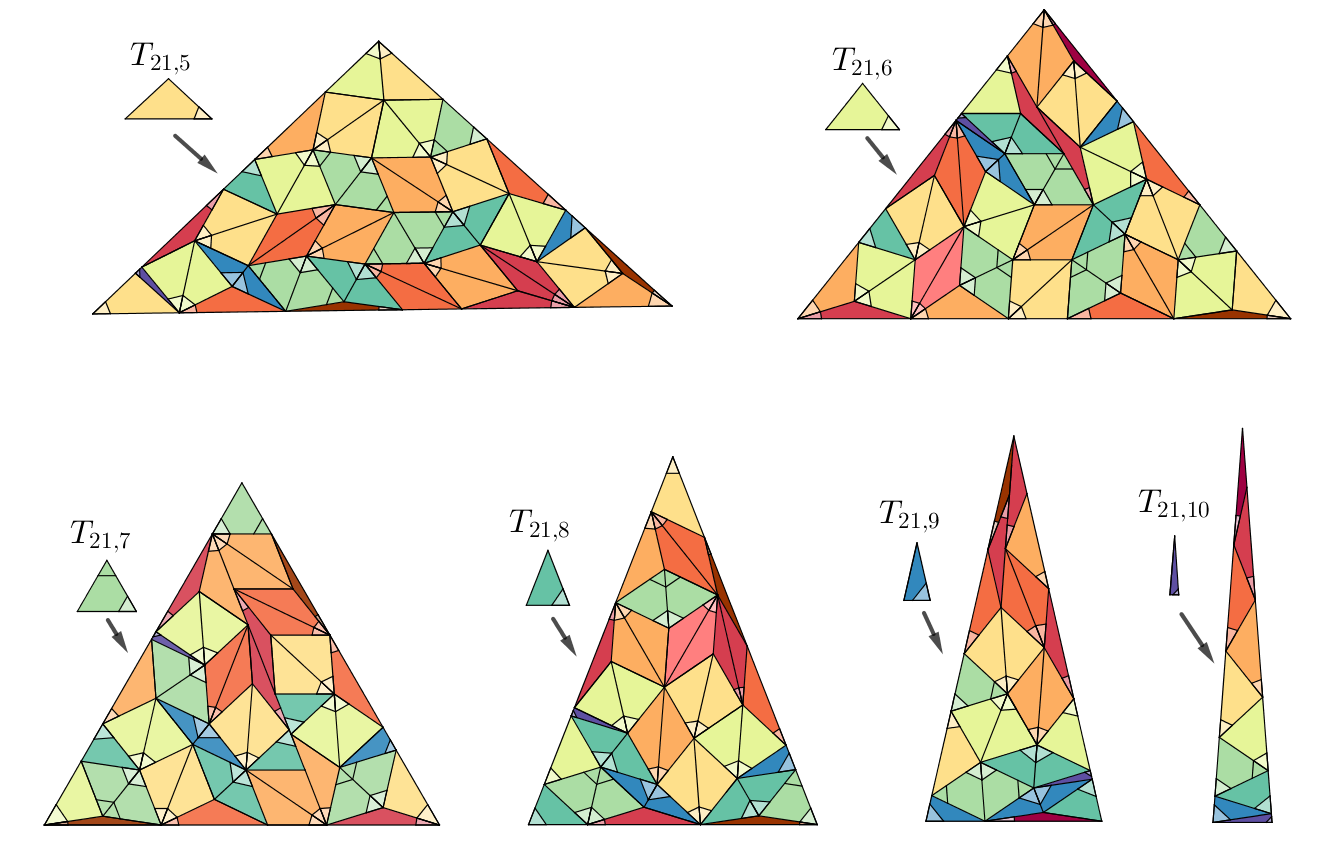
\includegraphics[width=.75\textwidth]{ILCFig5_21-fold_b_}\\
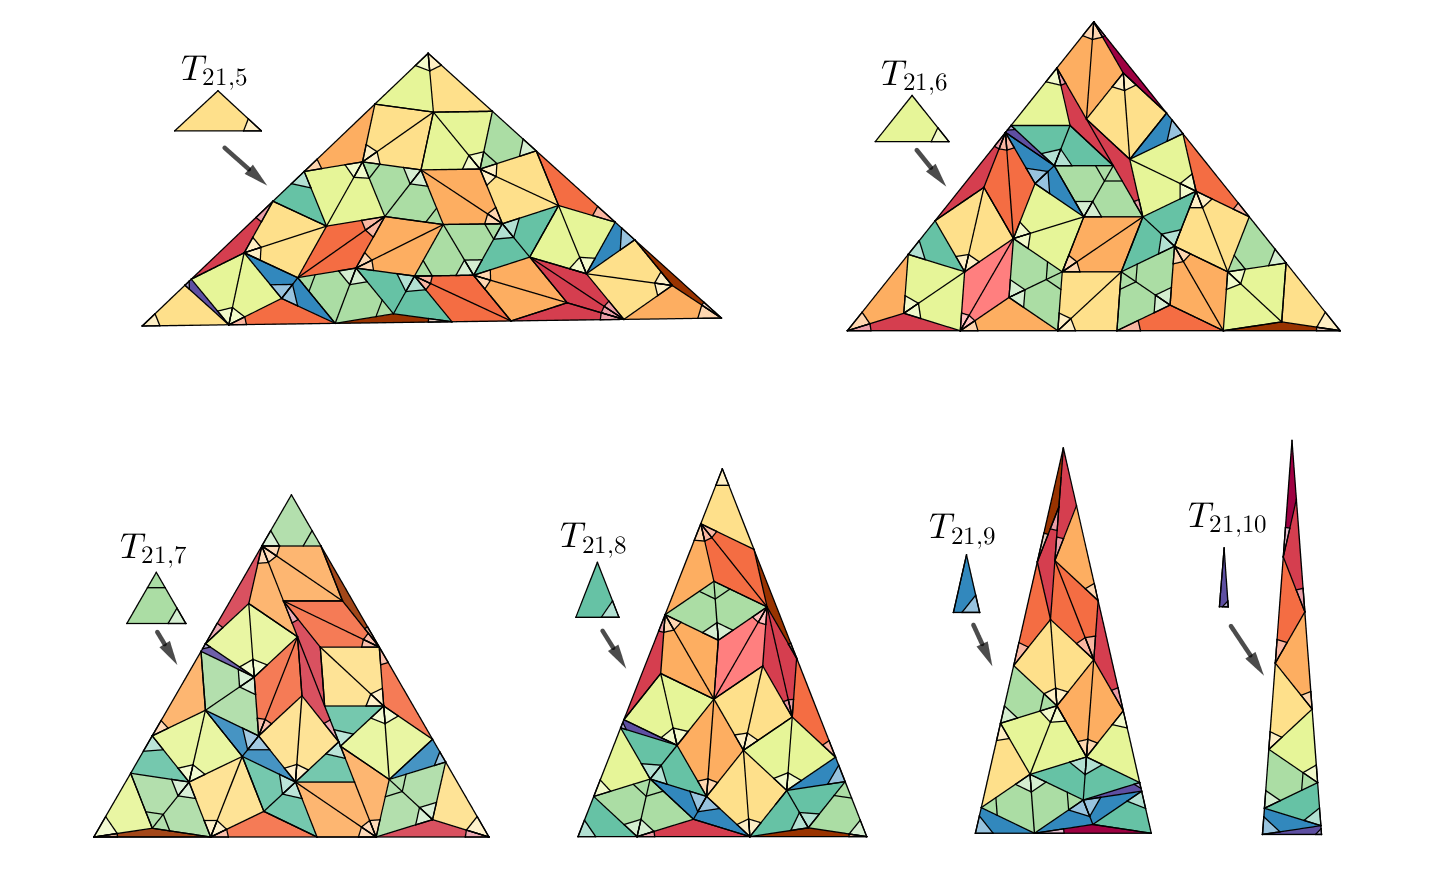
\includegraphics[width=.75\textwidth]{ILCFig5_21-fold_c_}
\caption{The substitution $\sigma_{21}$.  
\label{fig:21-fold}}
\end{figure}
\newpage

As in the case \( n = 13 \), the tiling spaces \(\mathbb{X}_{\sigma_{17}}\) and \(\mathbb{X}_{\sigma_{21}}\) contain tilings \(\mathcal{T}_{17}\) and \(\mathcal{T}_{21}\) with \(17\)-fold and \(21\)-fold rotational symmetry, respectively. The derivation of each tiling is analogous to that of \(\mathcal{T}_{13}\) described in the preliminaries. In each case, the tiling arises from the kite-shaped edge type at the right corner of \(\sigma_{n}(T_{n,2})\), identical to \(K\) in \(\sigma_{13}(T_{13,2})\).

\begin{figure}[H]
\centering
\includegraphics[width=1\textwidth]{ILCFig6_17-fold}
			\caption{A patch of the tiling $\mathcal{T}_{17}$. The tiles have been recolored for aesthetic purposes.}
\label{fig:17-fold-tiling}
\end{figure}

\begin{figure}[H]
\centering
\includegraphics[width=0.9\textwidth]{ILCFig7_21-fold}
			\caption{A patch of the tiling $\mathcal{T}_{21}$. }
\label{fig:21-fold-tiling}
\end{figure}

\newpage

\subsection{The KSK Criterion and Its Application to the Construction of $\sigma_n$}
\noindent We now discuss a useful tool---the KSK criterion---which we employed in deriving the substitution rules, in particular in the dissection of the inflated prototiles. This criterion has previously been used to generate substitution tilings with rhombic prototiles (see, for example, \cite{Mal15, KarRis16, Pau17}). Although the prototiles in the present work are triangles, the KSK criterion remains very useful, with the aim of dissecting the inflated prototiles so that isosceles triangles in certain regions of their interior meet along their bases to form rhombs.

The KSK criterion, developed independently by Kannan and Soroker~\cite{KanSor92} and by Kenyon~\cite{Ken93}, determines whether a given polygonal region~$\mathcal{R}$ can be tiled using parallelograms. Here, we assume that the boundary of $\mathcal{R}$ consists of edges of equal length, and hence the resulting parallelograms are rhombs.

The KSK criterion consists of two conditions, namely, the \textit{balance} and \textit{convex crossing} conditions. We describe the criterion using a concrete example~$\mathcal{R}$ shown in Fig.~\ref{fig:convex(a)}. To properly define these conditions, we view the boundary of~$\mathcal{R}$ as a set~$\mathcal{E}$ of oriented edges arranged in counterclockwise order starting from some fixed vertex (see Fig.~\ref{fig:convex(b)}). The first condition of the criterion is the following. \\

\noindent \textbf{Balance Condition:} The set~$\mathcal{E}$ can be partitioned into pairs of oriented edges with opposite directions.\\

We then join each pair using a smooth planar curve such that each crossing is formed by exactly two curves (see Fig.~\ref{fig:convex(b)}). Our next focus of investigation is on the crossings themselves. Let \(E_1 = \{e_1, e_1'\}\) and \(E_2 = \{e_2, e_2'\}\) be two pairs of edges whose corresponding curves cross, and suppose the sequence of oriented edges in counterclockwise order is given by 
$\ldots e_1 \ldots e_2 \ldots e_1' \ldots e_2' \ldots.$
We say that the pairs \(E_1\) and \(E_2\) have a \textit{convex crossing} if the angles subtended to the left of \(e_1\) and \(e_2\) (when the head of \(e_1\) is attached to the tail of \(e_2\) and the head of \(e_2\) to the tail of \(e_1'\), respectively) are less than \(\pi\). Equivalently, the oriented edges \(e_1, e_2, e_1', e_2'\) form a rhomb inside \(\mathcal{R}\) when the head of \(e_1\) is attached to the tail of \(e_2\), \(e_2\) to \(e_1'\), and \(e_1'\) to \(e_2'\), as illustrated in Fig.~\ref{fig:convex(c)}. With this, the second condition of the criterion is the following:\\

\noindent \textbf{Convex Crossing Condition} Every pair of curves that cross must have a convex crossing.\\

If the two conditions are satisfied, then \(\mathcal{R}\) can be dissected into rhombs. The dissection is carried out by noting that each smooth planar curve corresponds to a chain of rhombs, as illustrated in Fig.~\ref{fig:convex(d)}.

\begin{figure}[H]
		\begin{subfigure}{0.45\textwidth}
			\centering
			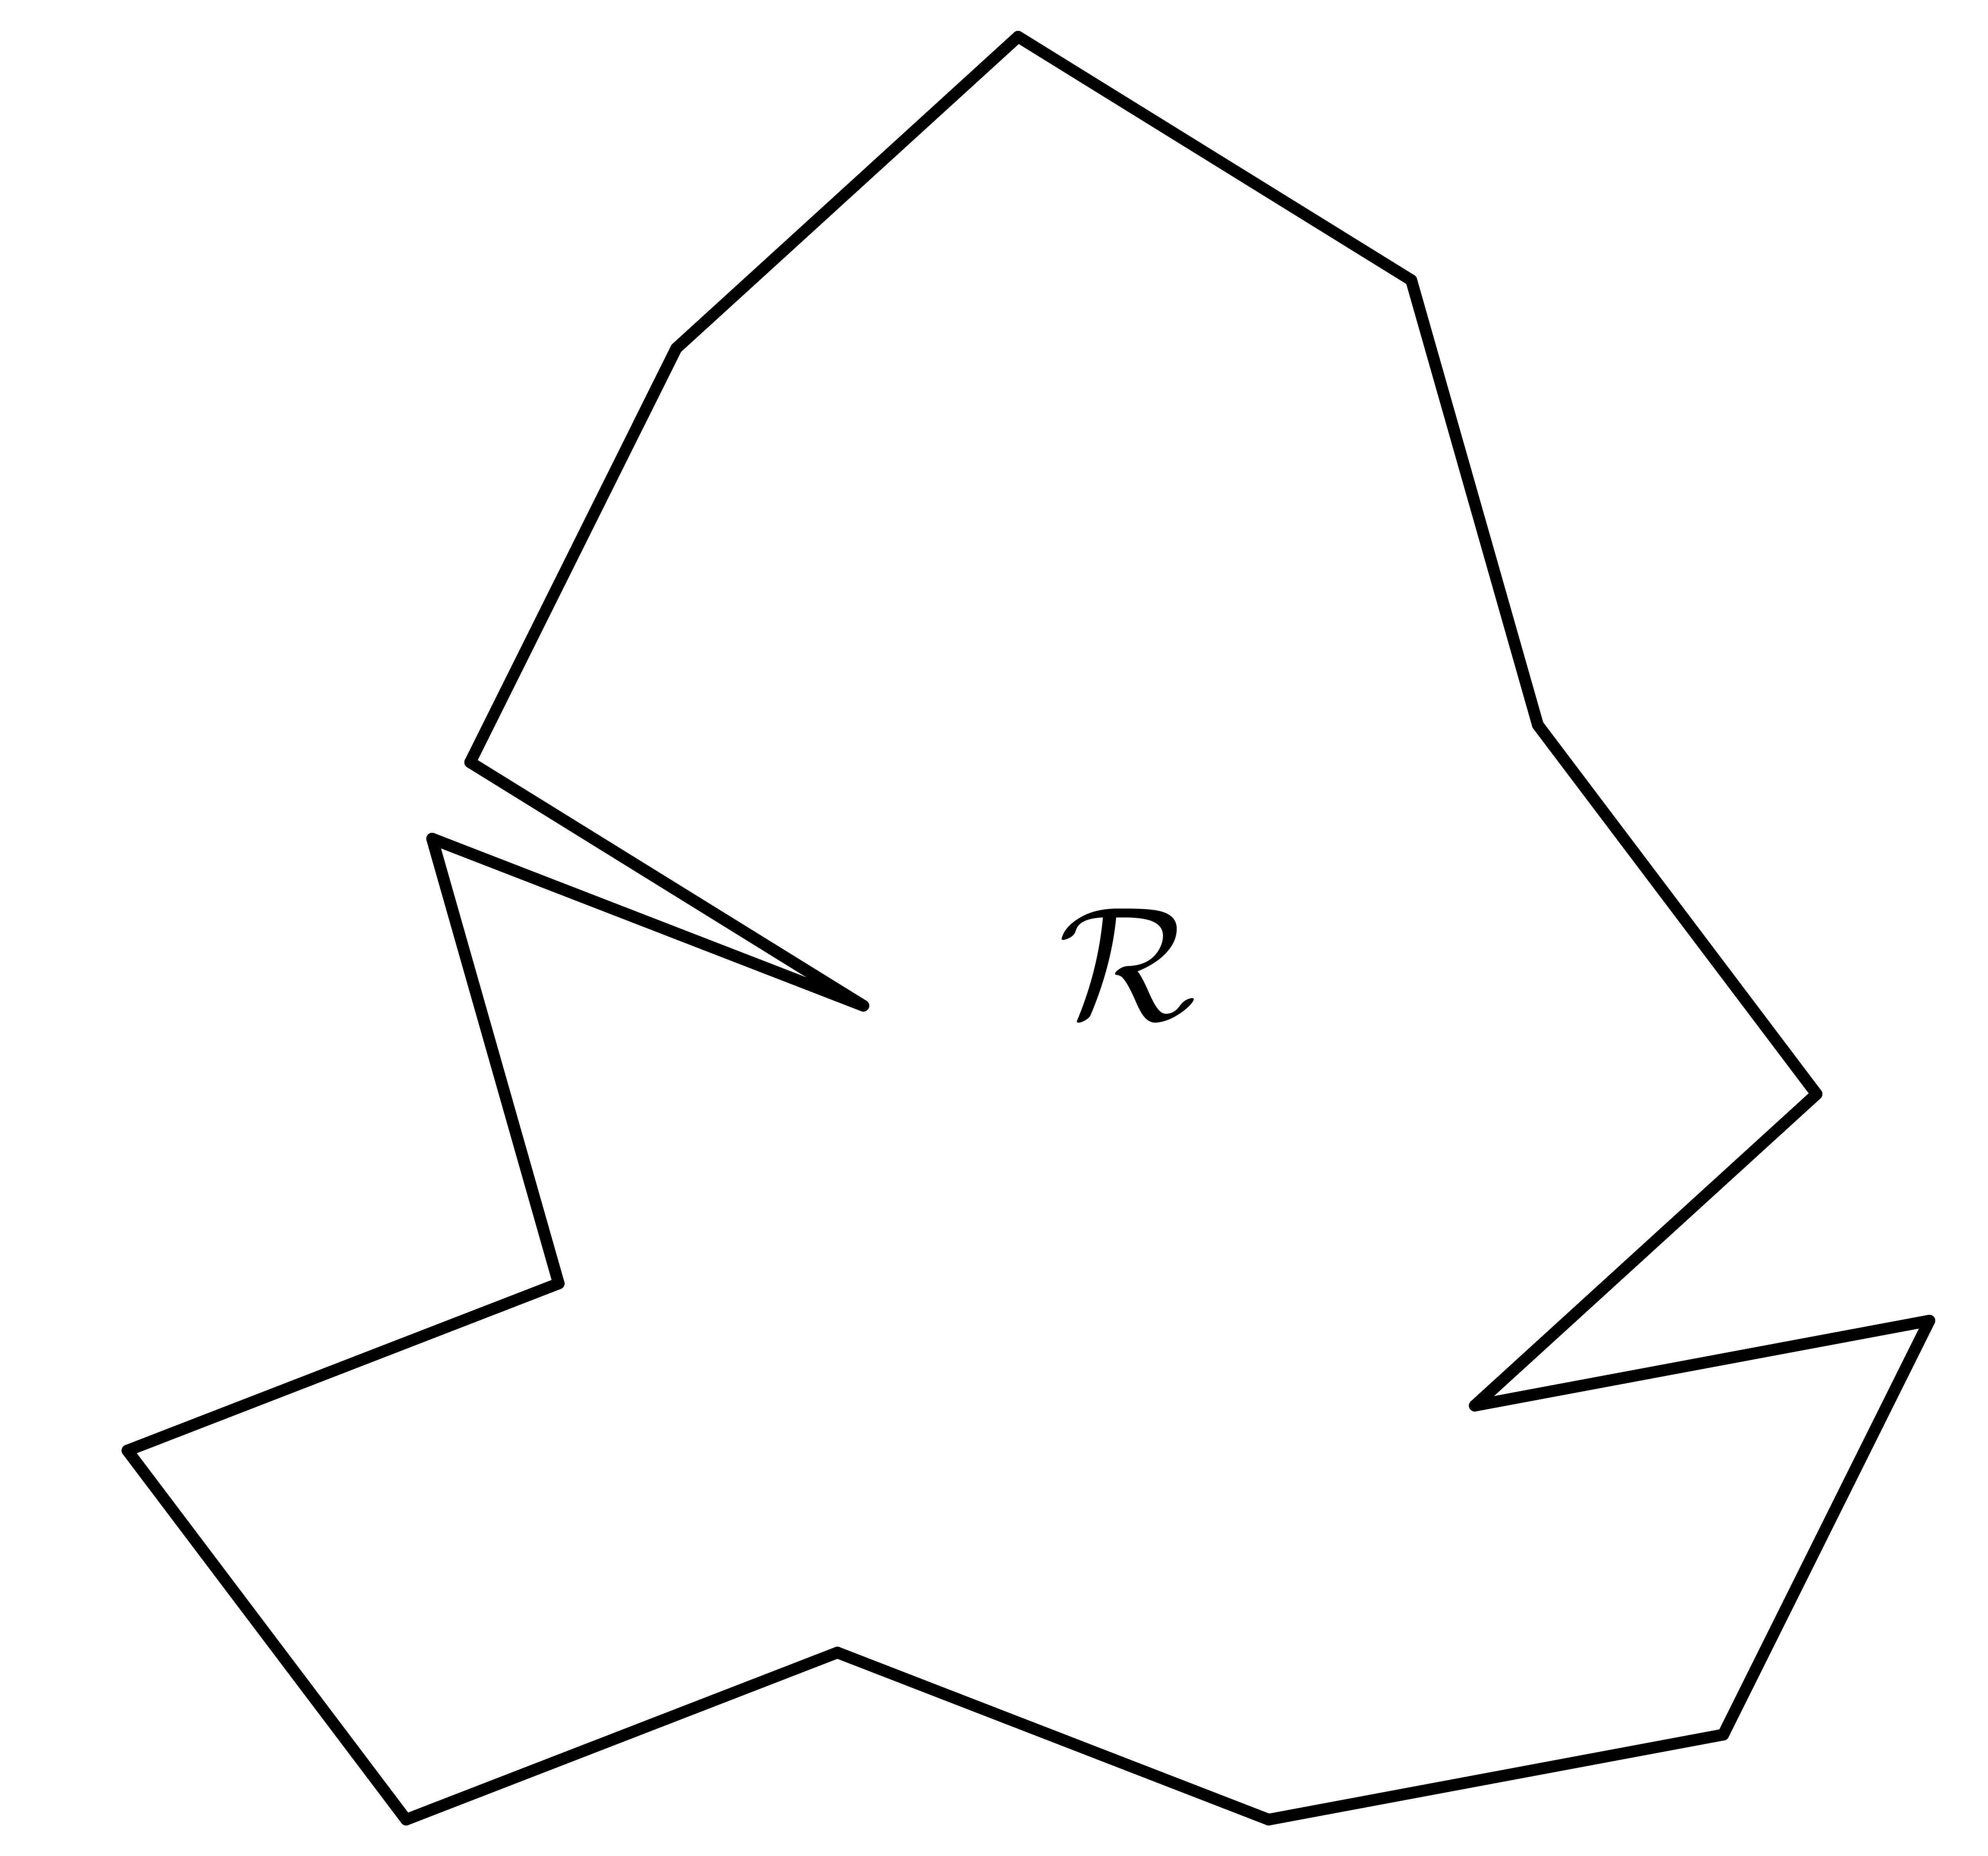
\includegraphics[scale=.12]{ILCFig8_region_a_}
			\caption{}
\label{fig:convex(a)}
		\end{subfigure}
		% Subfigure (b)
		\begin{subfigure}{0.45\textwidth}
			\centering
			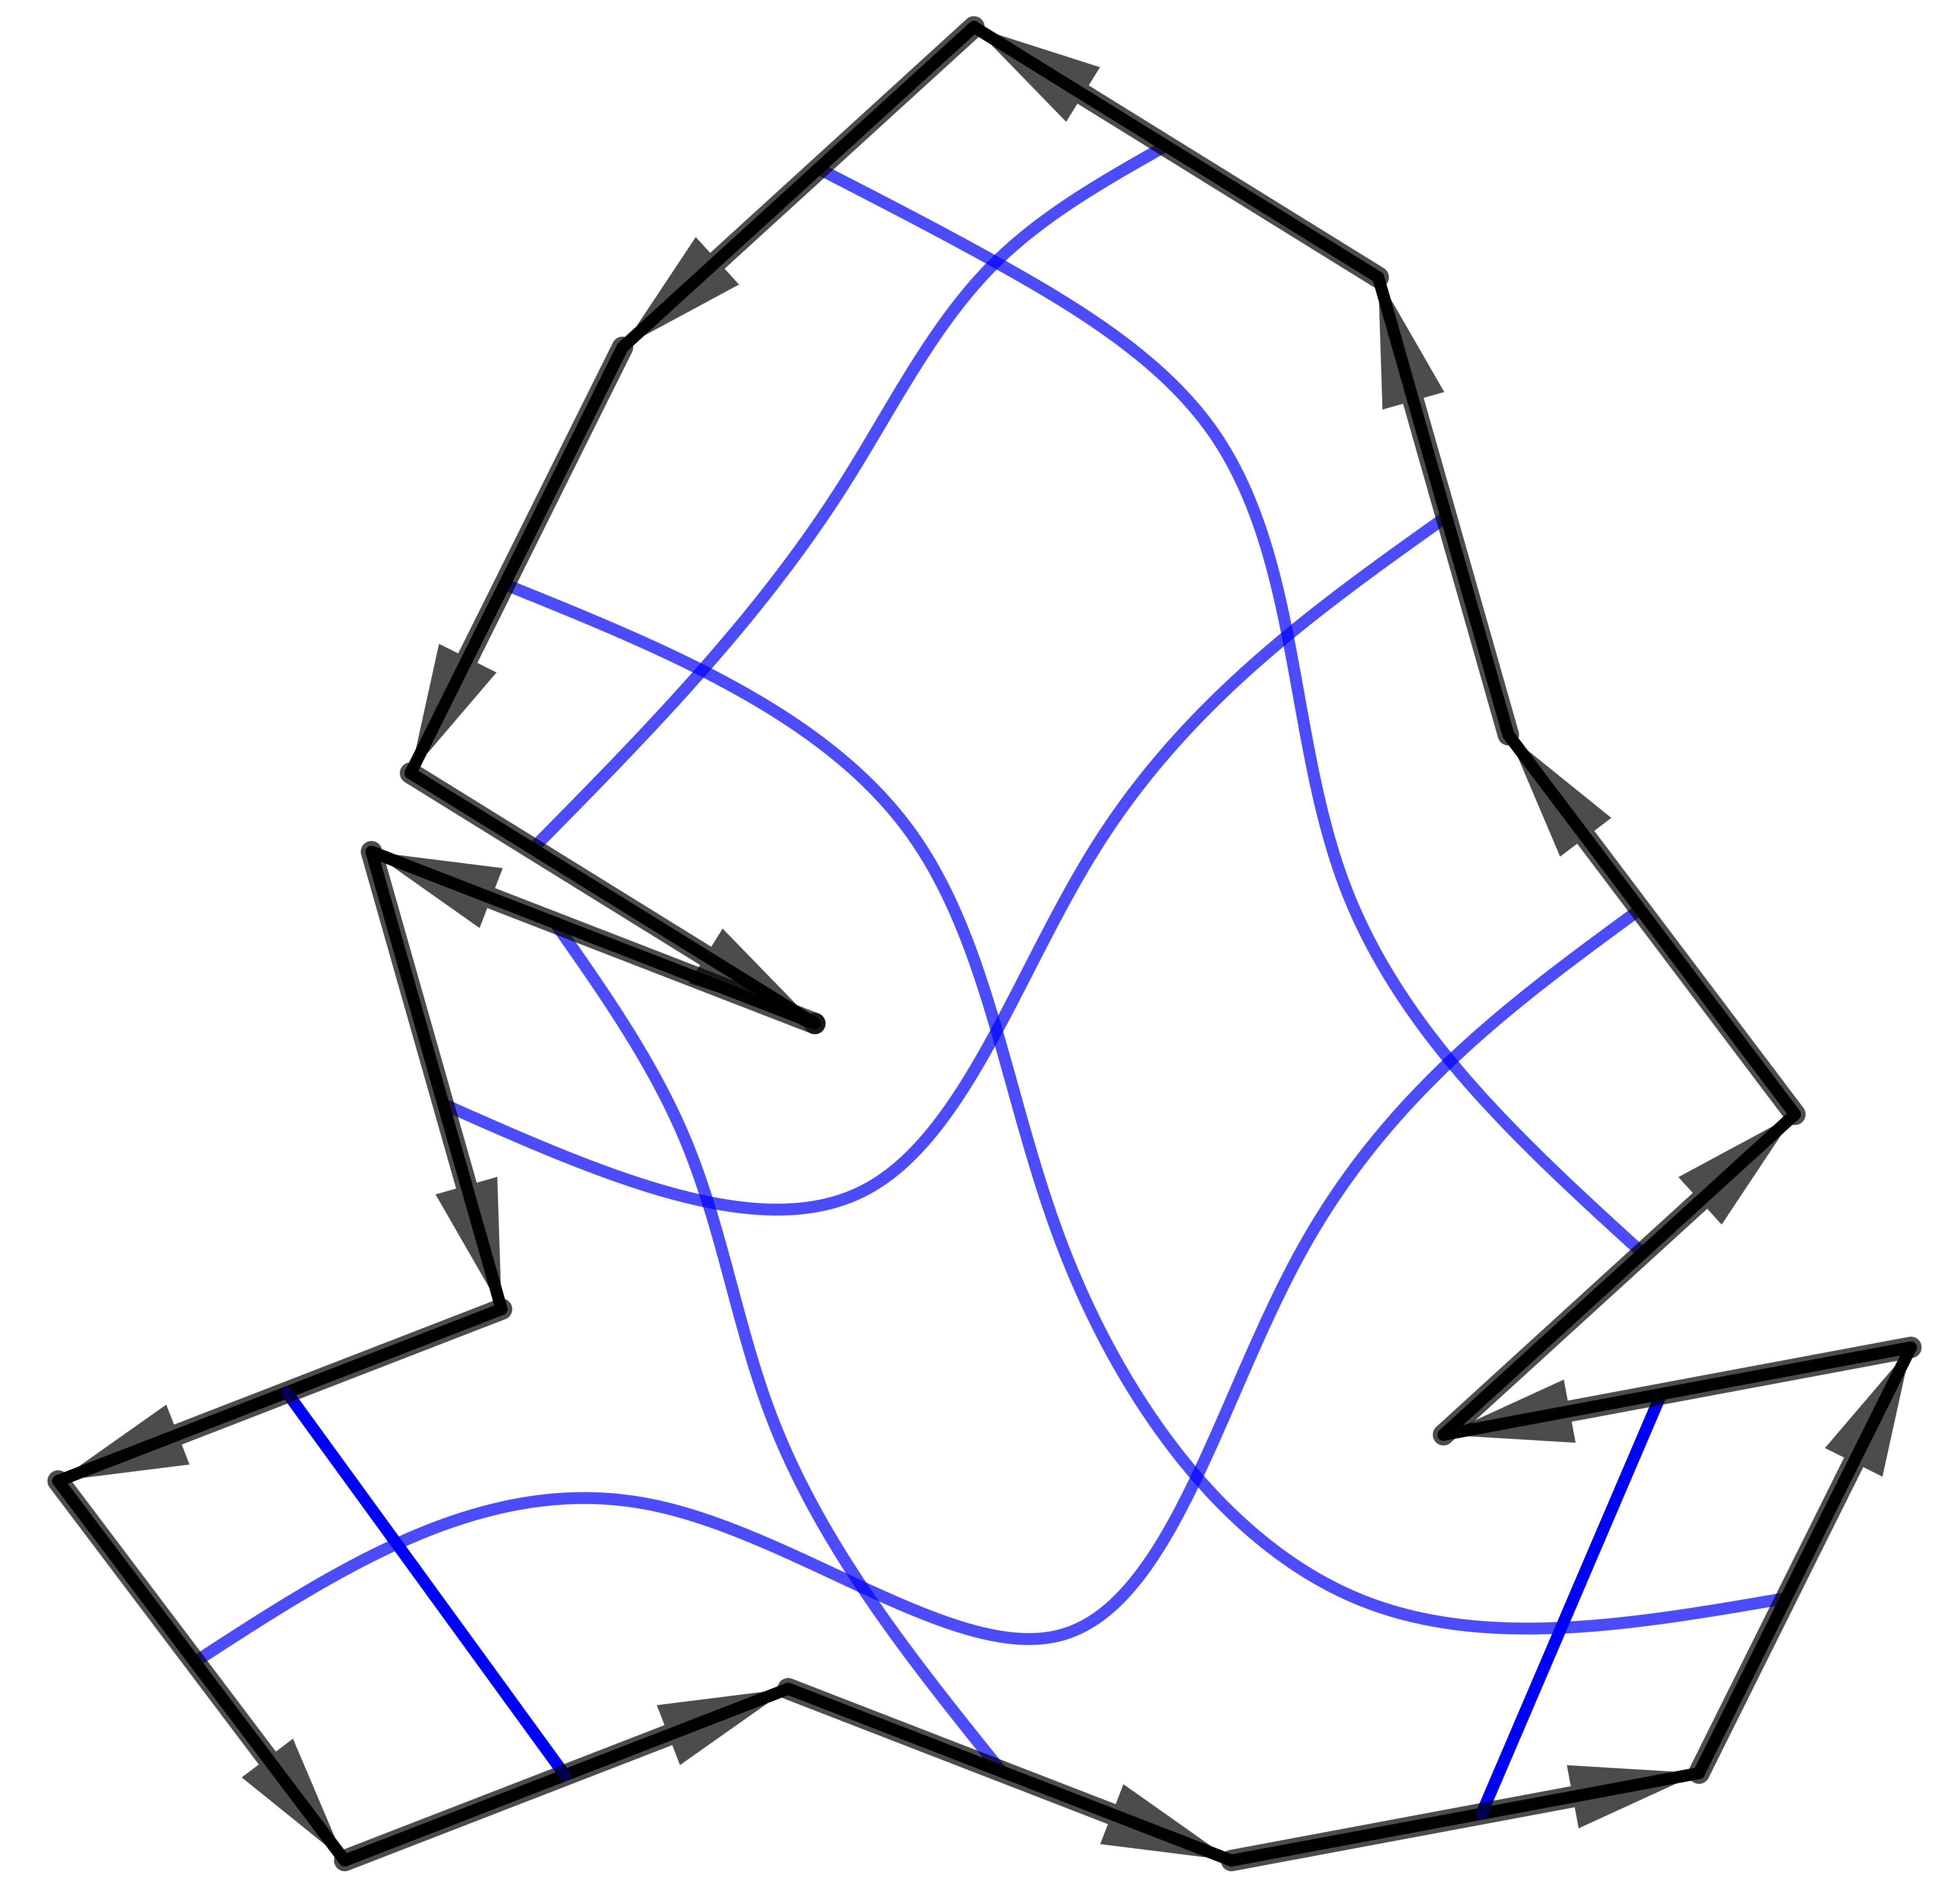
\includegraphics[scale=.12]{ILCFig8_region_b_}
			\caption{}
\label{fig:convex(b)}
		\end{subfigure} \\
		
		\begin{subfigure}{0.45\textwidth}
			\centering
			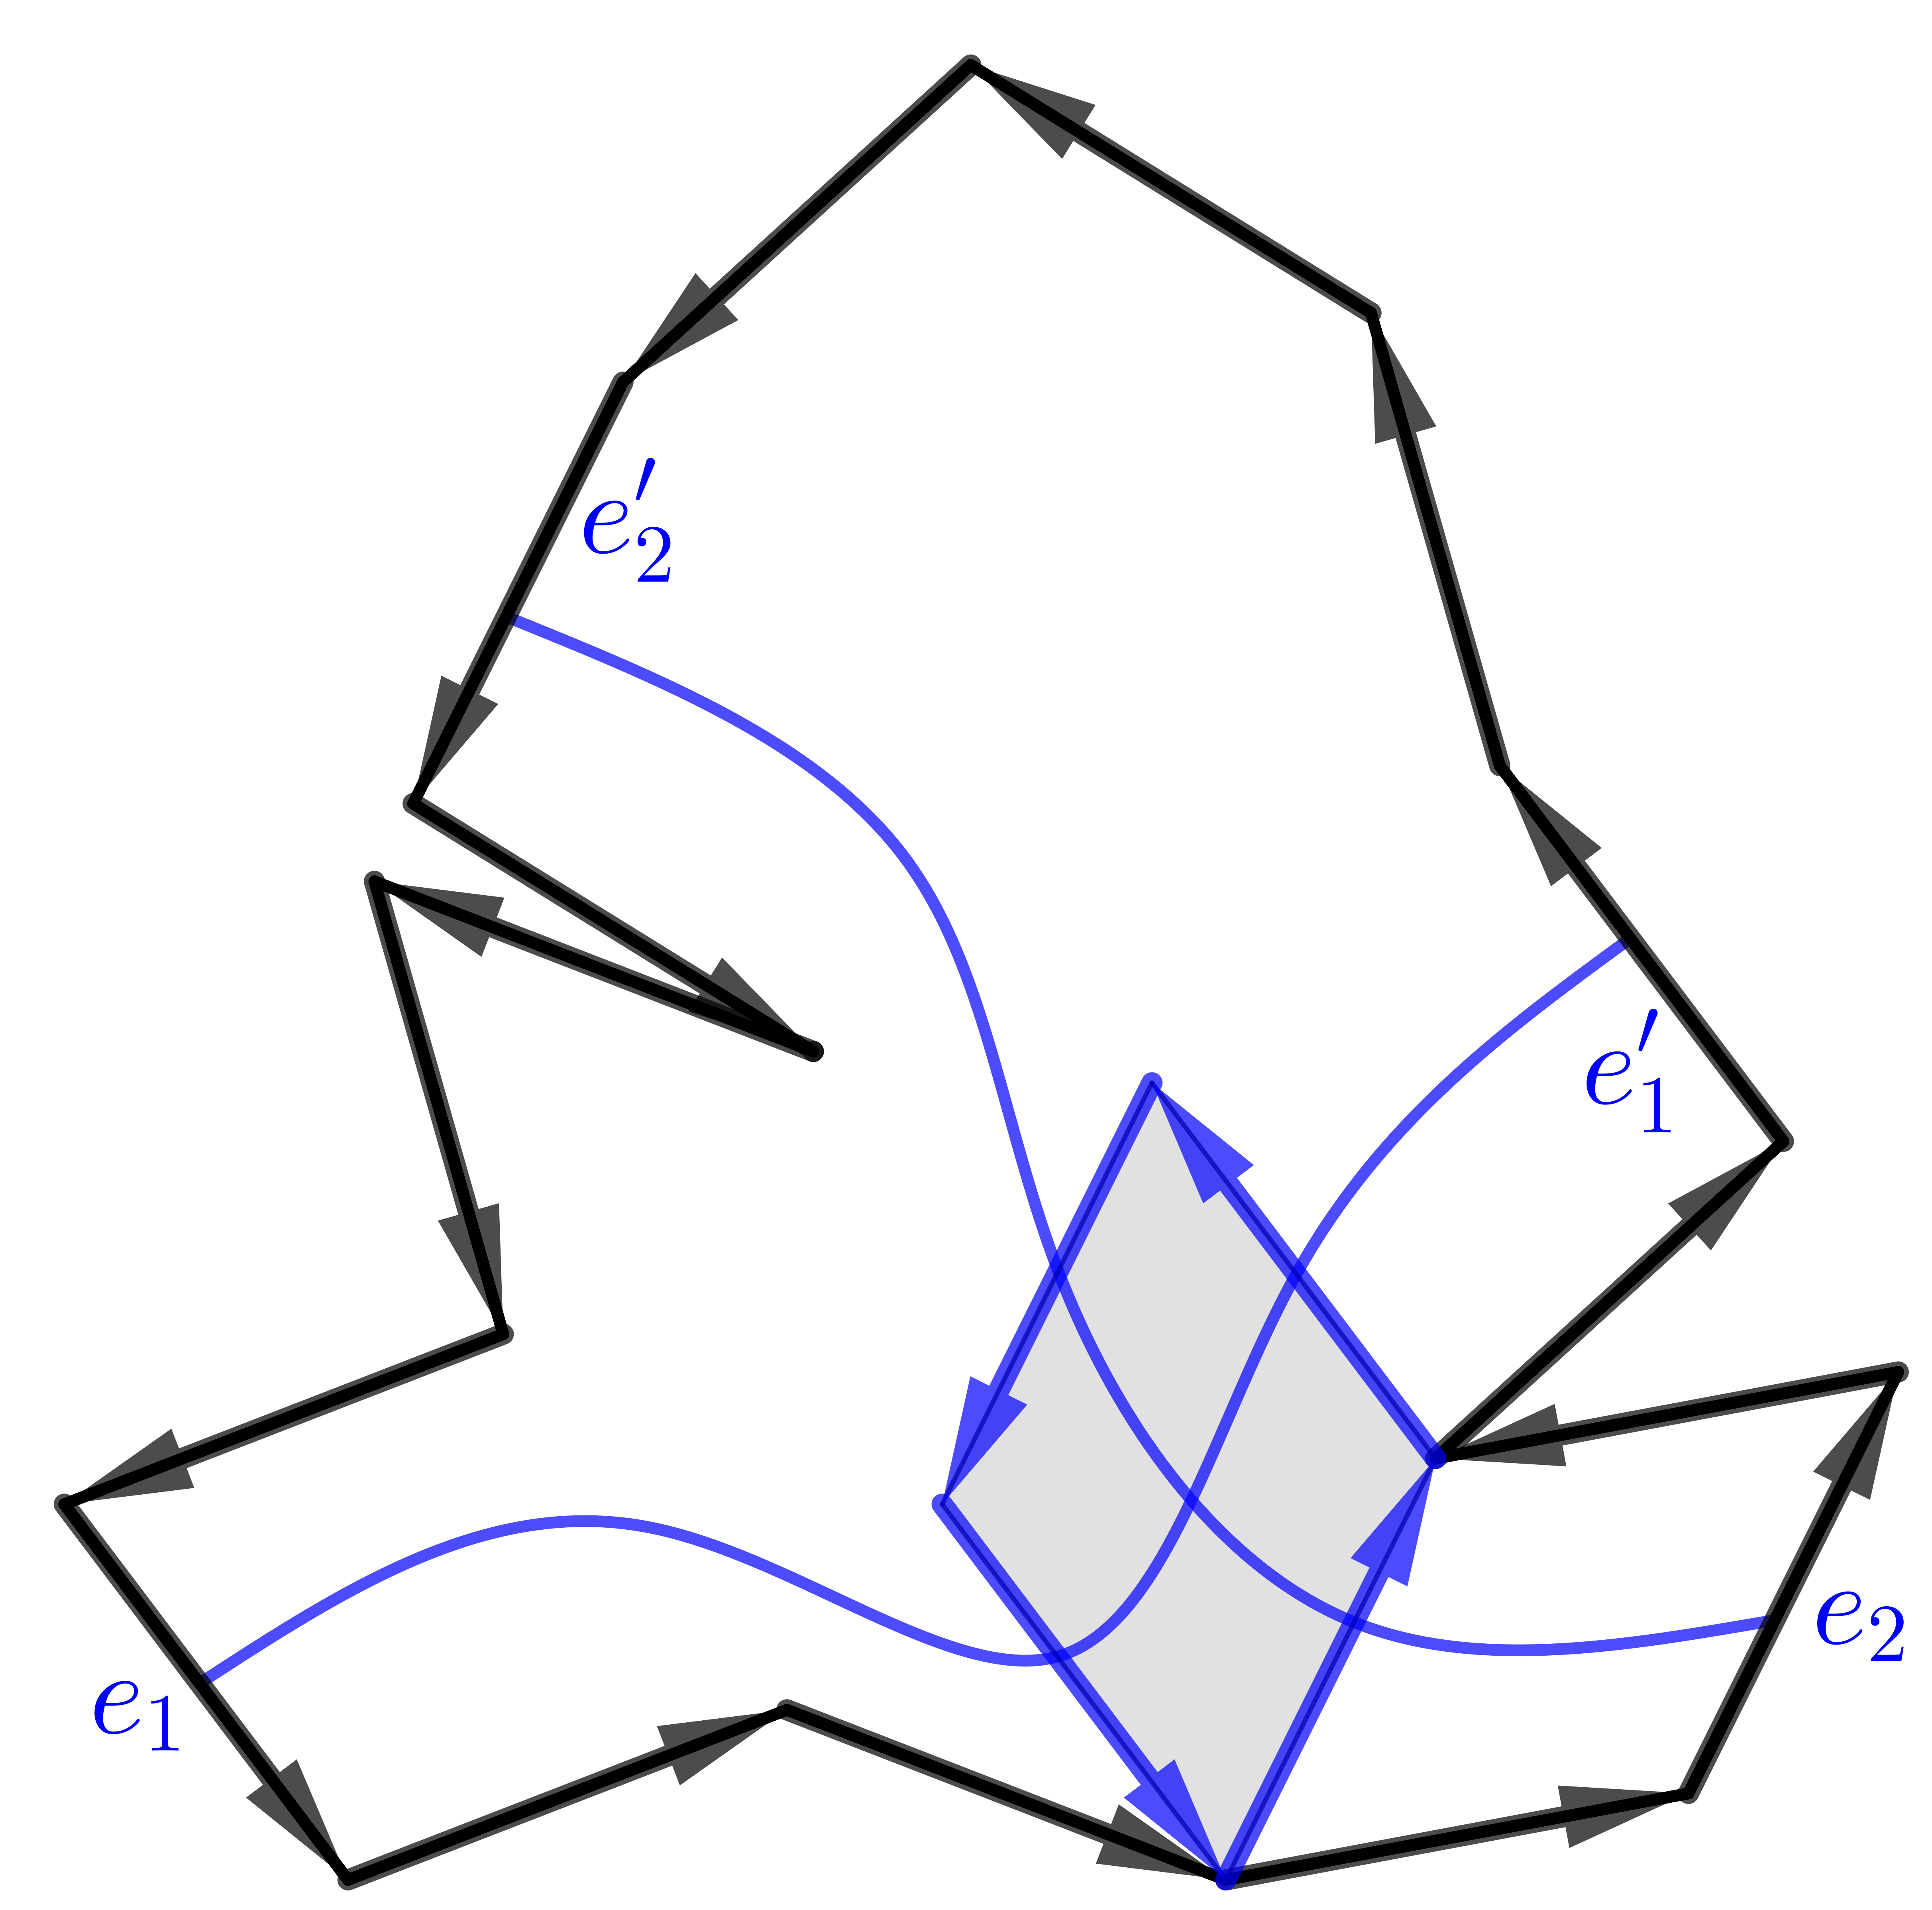
\includegraphics[scale=.12]{ILCFig8_region_c_}
			\caption{}
\label{fig:convex(c)}
		\end{subfigure}
		% Subfigure (b)
		\begin{subfigure}{0.45\textwidth}
			\centering
			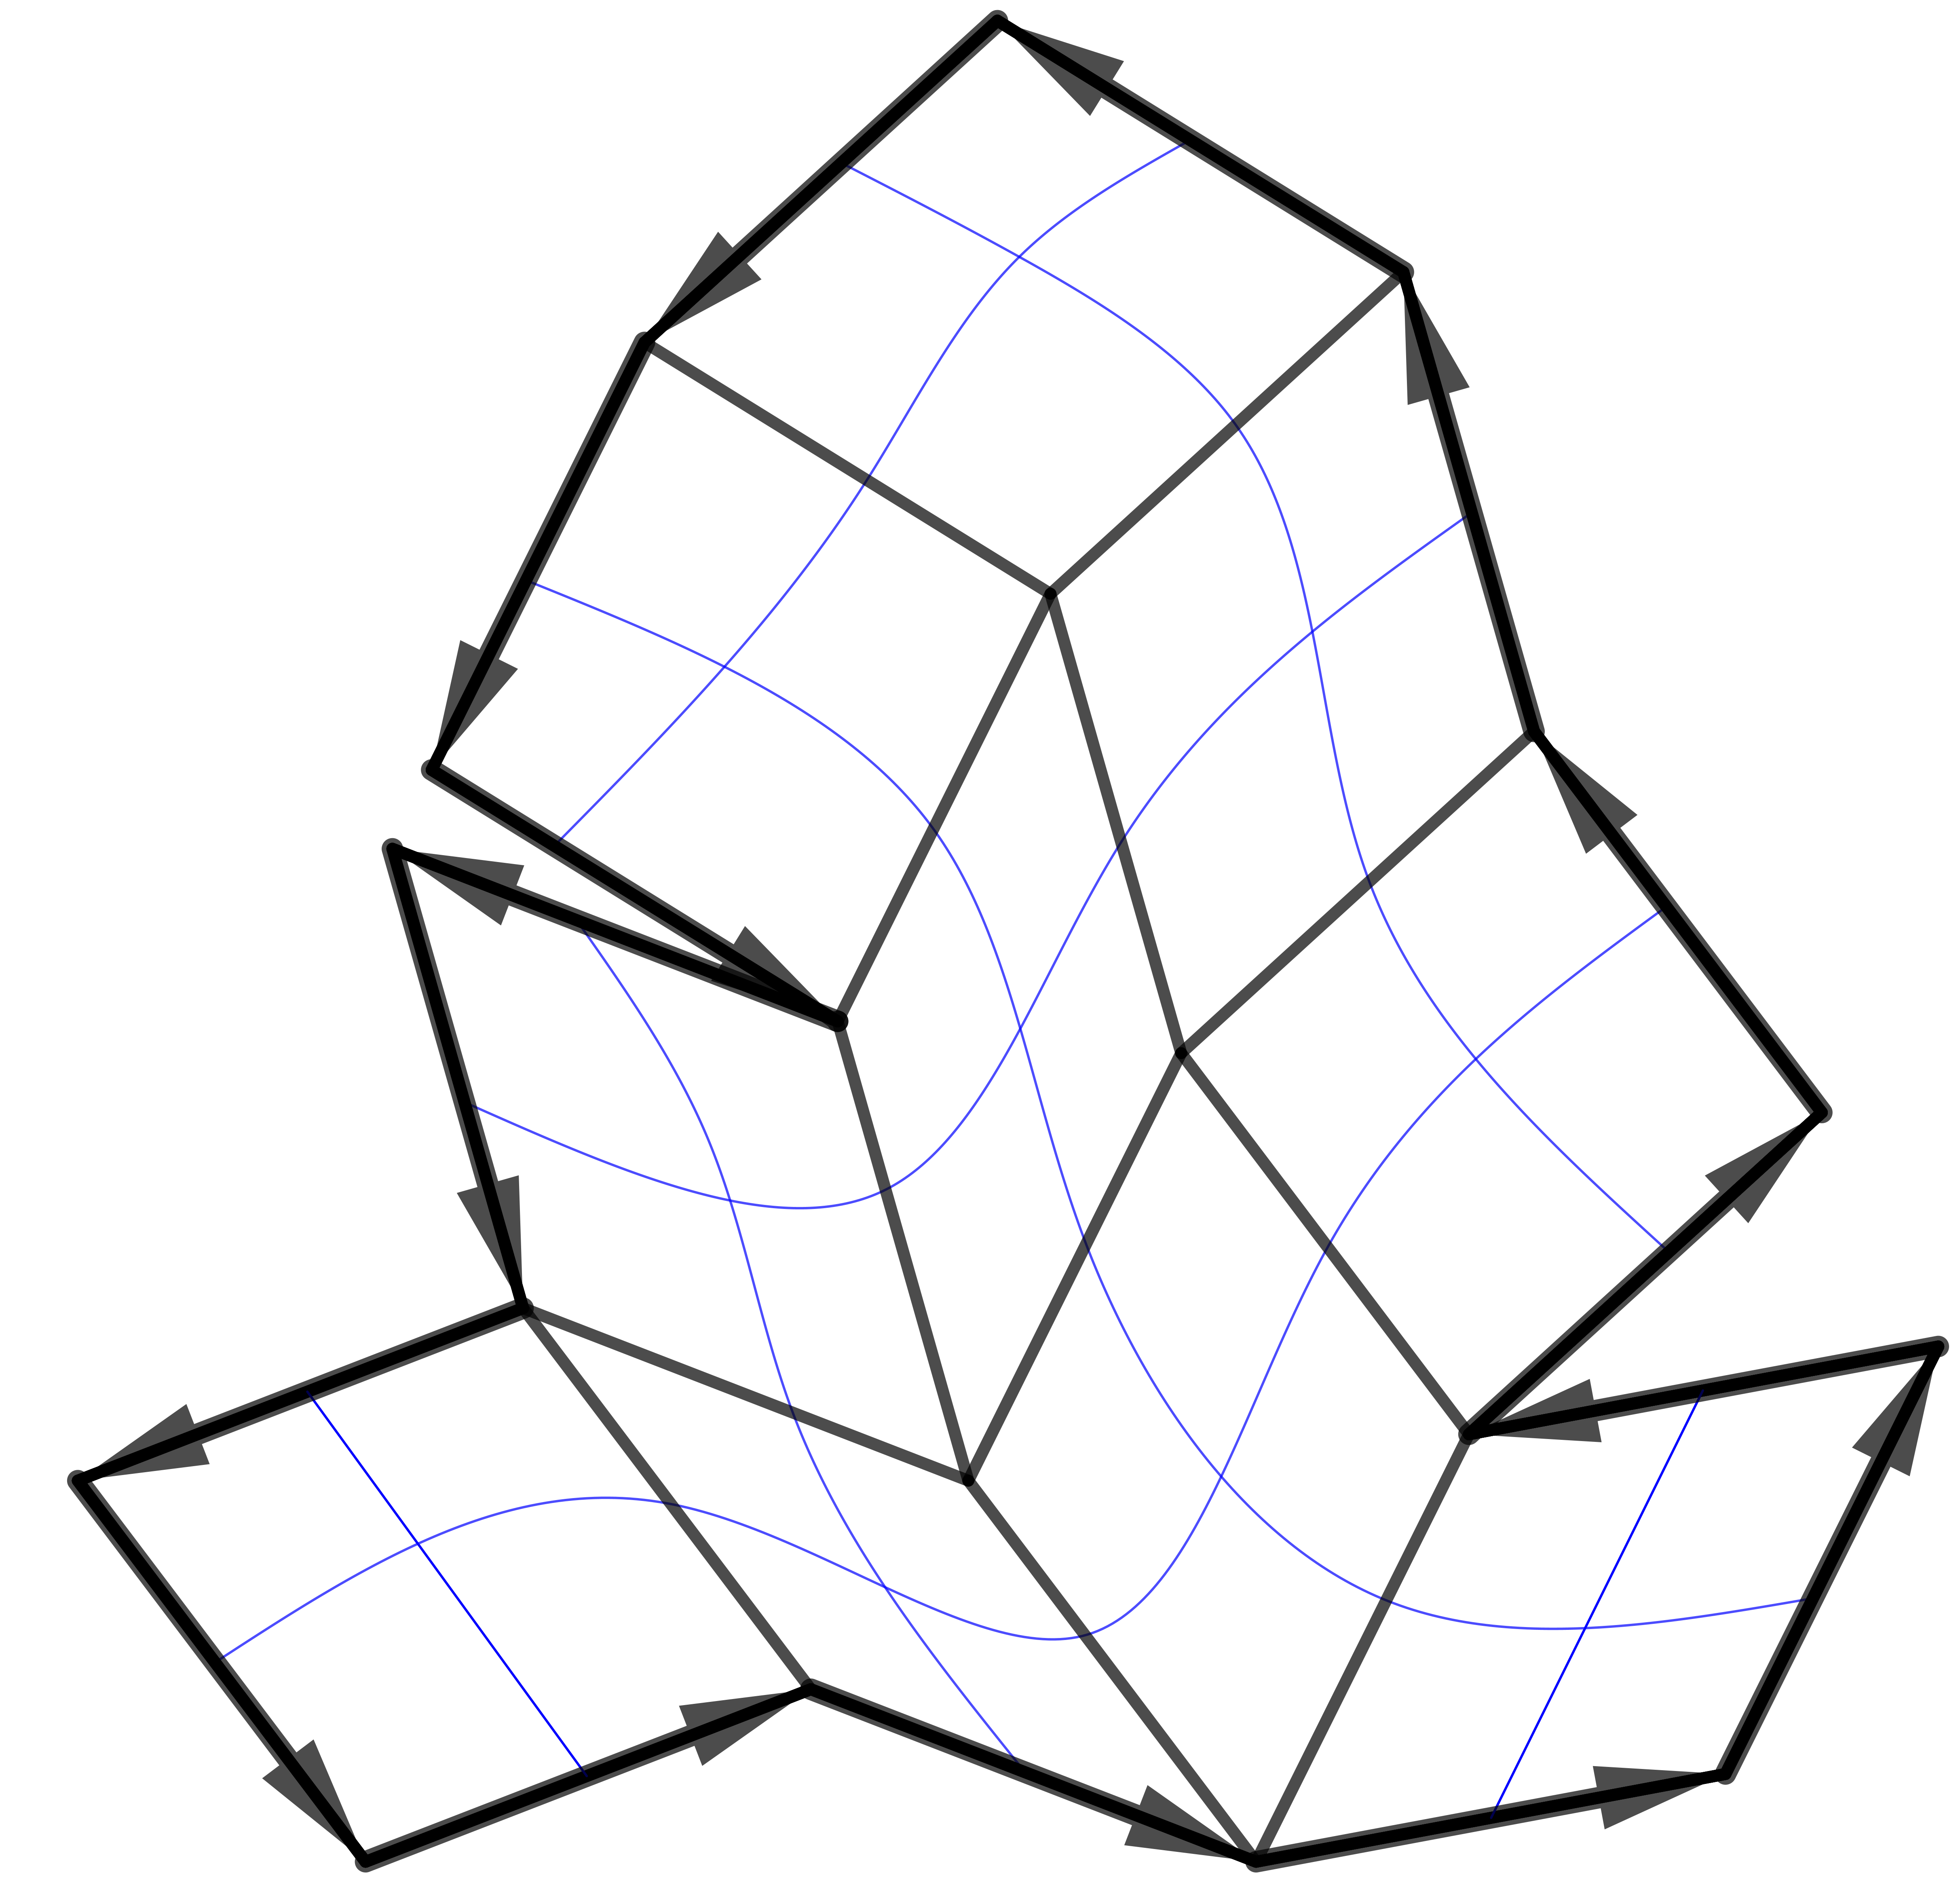
\includegraphics[scale=.12]{ILCFig8_region_d_}
			\caption{}
\label{fig:convex(d)}
		\end{subfigure}


		\caption{A region that satisfies the KSK criterion.}
		\label{fig:convex}
	\end{figure}

\subsubsection{The Dissection of $\mu_{17}T_{17,6}$}
We note that for any (self‐similar) substitution rule to be well‐defined, the lengths of the inflated sides of the prototiles (obtained by multiplying by the inflation factor) must be expressible as non‐negative integer linear combinations of the prototile edge lengths.

To describe the representations of $\mu_n$ and $\mu_n s_{n,k}$ as sums of $s_{n,j}$, we define
\[
I_n = \{0, 1, 2, \dots, (n-1)/2\}, \quad
I_{n,O} = I_n \cap (2\mathbb{Z}+1), \quad
I_{n,E} = I_n \cap 2\mathbb{Z}.
\]

For each $n \in \{13,17,21\}$, it can be verified that
\begin{equation}
\mu_n = \sum_{j \in I_{n,O}} s_{n,j} \;=\; \sum_{j \in I_{n,E}} s_{n,j},
\label{eq:legrep}
\end{equation}
and
\begin{equation}
\mu_n s_{n,k} = \sum_{j=0}^{\frac{\,n-1\,}{2} - k} s_{n,j}.
\label{eq:baserep}
\end{equation}
These equalities hold for every odd $n \ge 5$ and follow from the identity $(*)$ in~\cite{NisDanz96}.

To illustrate how to obtain a dissection of \(\mu_{n} T_{n,k}\) with the aid of the KSK criterion, we consider the case \(n = 17\) and \(k = 6\).

We define \(T_{17,0}\) as the horizontal segment of length \(s_{17,0} = 1\), and refer to it as a \textit{pseudo-prototile}. An equivalent copy of \(T_{17,0}\) is any isometric image of this segment. Whenever we refer to the \textit{base} or \textit{leg} of \(T_{17,0}\), we simply mean the segment itself.

Using the representations of \(\mu_{17}\) and \(\mu_{17} s_{17,6}\) given in Equations~\ref{eq:legrep} and~\ref{eq:baserep}, each edge of \(\mu_{17} T_{17,6}\) can be dissected into smaller segments, each of length \(s_{17,j}\), where \(j \in I_{17} = \{0, 1, 2, \ldots, 8\}\).  We define the dissection of the left leg using  
$\mu_{17} = s_{17,0} + s_{17,2} + s_{17,4} + s_{17,8},$ and the right leg using $\mu_{17} = s_{17,1} + s_{17,3} + s_{17,5} + s_{17,7}.$ The base is dissected using $s_{17,0} + s_{17,1} + s_{17,2}.$

Noting that \(s_{17,j}\) is the length of the base of the prototile \(T_{17,j}\), we place, for each small edge of length \(s_{17,j}\), a tile equivalent to \(T_{17,j}\) inside the inflated prototile so that its base coincides with the small edge. In this way, any edge dissection \(\mathcal{D}_{17,6}\) determines the tile types along the boundary of \(\mu_{17} T_{17,6}\). Specifically:  
\begin{enumerate}
\item[-] The left leg contains one copy each of \(T_{17,0}, T_{17,2}, T_{17,4}, T_{17,8}\);  
\item[-] The right leg contains one copy each of \(T_{17,1}, T_{17,3}, T_{17,5}, T_{17,7}\);  
\item[-] The base contains one copy each of \(T_{17,0}, T_{17,1}, T_{17,2}\).  
\end{enumerate}

The question now is: how should \(\mathcal{D}_{17,6}\) be chosen to ensure that the inflated triangle \(\mu_{17} T_{17,6}\) can be dissected into copies of the prototiles? An obvious restriction on \(\mathcal{D}_{17,6}\) is that the initial (boundary) tiles must have pairwise disjoint interiors and must lie entirely within the large triangle \(\mu_{17} T_{17,6}\). For instance, the tile equivalent to \(T_{17,8}\) on the left side of \(\mu_{17} T_{17,6}\) cannot be placed at a corner; otherwise, part of it would lie outside the large triangle (see Fig.~\ref{fig:wrongarr}). Beyond these geometric constraints, the KSK criterion is crucial for identifying admissible choices of \(\mathcal{D}_{17,6}\).

\begin{figure}[H]
  \centering
  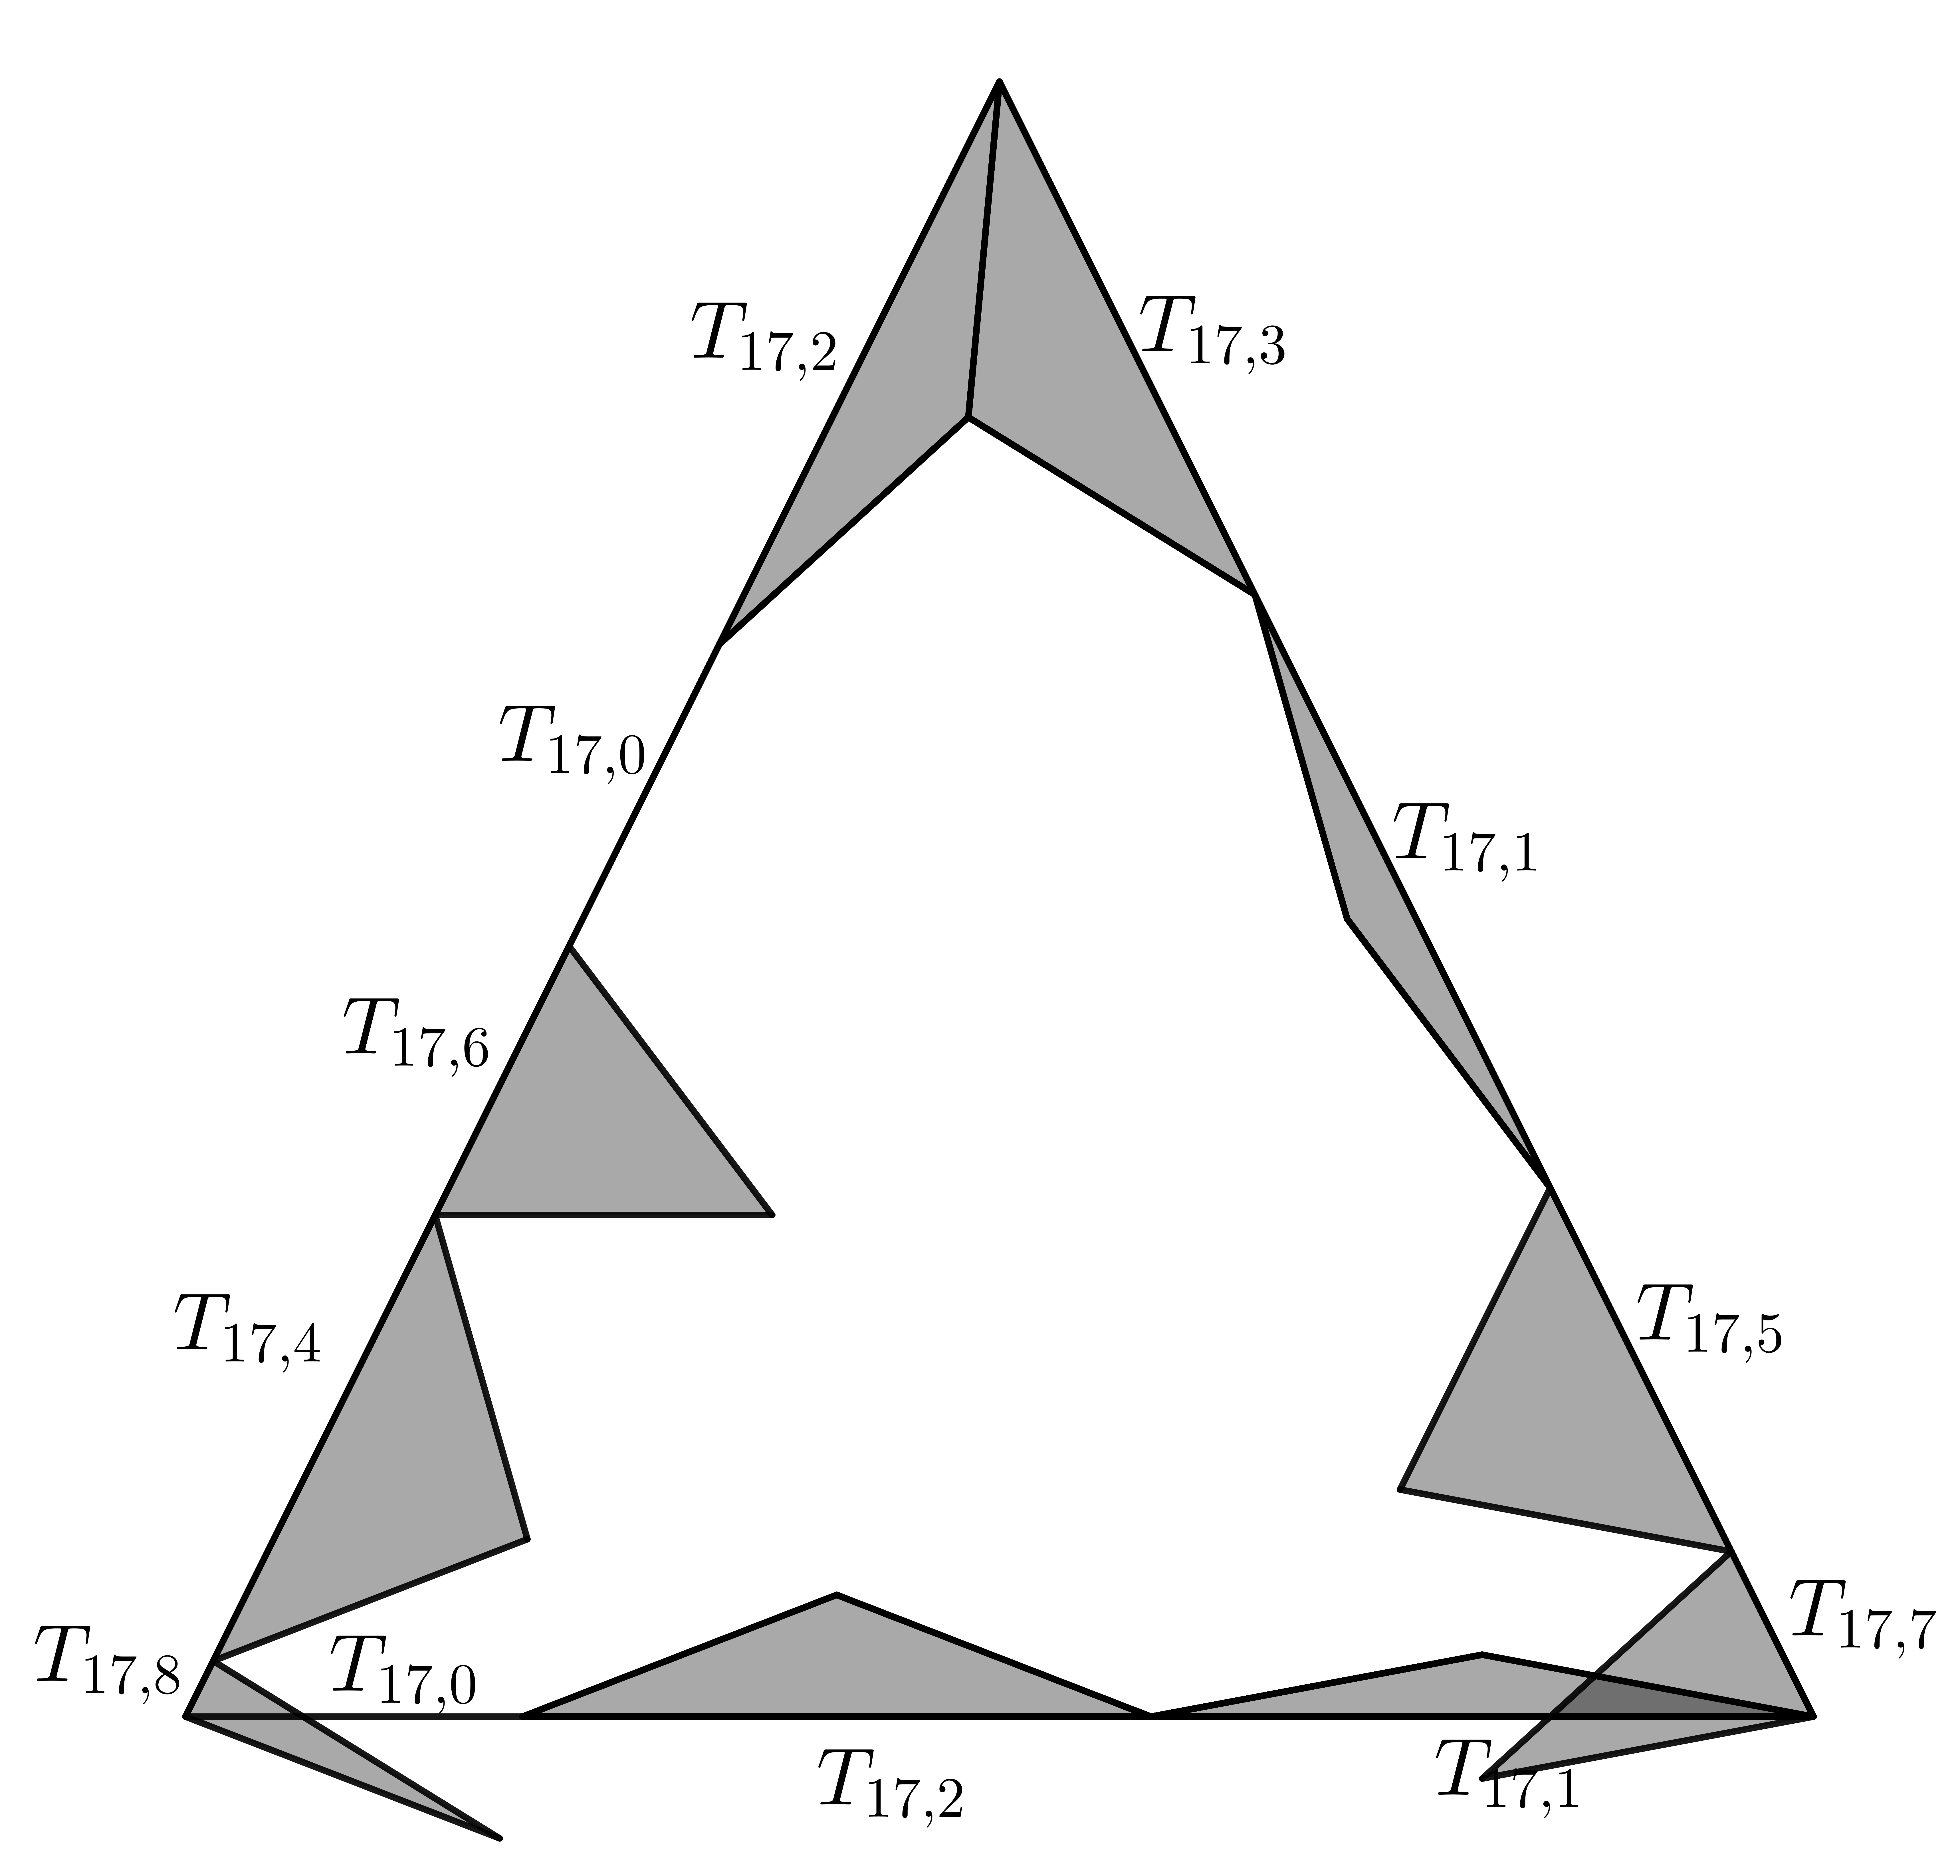
\includegraphics[scale=.11]{ILCFig9_wrongarr}
  \caption{An inadmissible arrangement of tiles along the boundary.}
  \label{fig:wrongarr}
\end{figure}

At this stage, \(\mathcal{D}_{17,6}\) is not yet specified. For any given choice of \(\mathcal{D}_{17,6}\), let \(R_{17,6}\) denote the region that remains to be dissected after placing the corresponding initial tiles along the boundary of \(\mu_{17} T_{17,6}\). Our objective is to determine \(\mathcal{D}_{17,6}\) so that the resulting \(R_{17,6}\) satisfies the KSK criterion.

We begin by assigning orientations to the legs of the initial tiles in a counterclockwise direction. We then show that, for any choice of \(\mathcal{D}_{17,6}\), the corresponding region \(R_{17,6}\) satisfies the balance condition. Table~\ref{tab:labels} lists the prototiles that appear along each side of \(\mu_{17} T_{17,6}\), together with the positive angles their legs make with the \(x\)-axis. As shown in the table, all these angles are distinct and can be partitioned into pairs, as detailed in Table~\ref{tab:partition}, where the difference between the angles in each pair is either \(\pi\) or \(-\pi\), indicating opposite directions. For example, the left leg of the copy of \(T_{17,2}\) on the left side of the large triangle is paired with the right leg of the copy of \(T_{17,3}\) on the right side, since $\frac{25\pi}{17} - \frac{8\pi}{17} = \frac{17\pi}{17} = \pi.$

Matched edges may either overlap completely or appear as edges of the boundary of the undissected region \(R_{17,6}\). The oriented edges of the boundary of \(R_{17,6}\) are precisely those that do not overlap, yet can still be grouped into pairs of oriented edges with opposite directions. Hence, the balance condition is satisfied.

\begin{center}
\renewcommand{\arraystretch}{1.5}
\captionof{table}{Prototiles that appear along the sides of $\mu_{17}T_{17,6}$ and the angles $s\pi/17$ made by the left (L) and right (R) legs of the tiles with the positive $x$-axis, measured counterclockwise.}
\label{tab:labels}
\begin{tabular}{| c | l | c | l | c | l |}
\hline
Left & Angles & Right & Angles & Base & Angles \\
& $L, R$ & & $L, R$ & & $L, R$ \\
\hline
$T_{17,0}$ & $\frac{23\pi}{17}$ & $T_{17,1}$ & $\frac{12\pi}{17}, \frac{10\pi}{17}$ & $T_{17,0}$ & $0$ \\
$T_{17,2}$ & $\frac{25\pi}{17}, \frac{21\pi}{17}$ & $T_{17,3}$ & $\frac{14\pi}{17}, \frac{8\pi}{17}$ & $T_{17,1}$ & $\frac{\pi}{17}, \frac{33\pi}{17}$ \\
$T_{17,4}$ & $\frac{27\pi}{17}, \frac{19\pi}{17}$ & $T_{17,5}$ & $\frac{16\pi}{17}, \frac{6\pi}{17}$ & $T_{17,2}$ & $\frac{2\pi}{17}, \frac{32\pi}{17}$ \\
$T_{17,6}$ & $\frac{29\pi}{17}, \pi$ & $T_{17,7}$ & $\frac{18\pi}{17}, \frac{4\pi}{17}$ & & \\
$T_{17,8}$ & $\frac{31\pi}{17}, \frac{15\pi}{17}$ & & & & \\
\hline
\end{tabular}
\end{center}


\begin{center}
\renewcommand{\arraystretch}{1.5}
\captionof{table}{Pairs of angles that differ by $\pm \pi$.}
\label{tab:partition}
\begin{tabular}{| c | c | c | c | c | c | c | c | c | c | c | }
\hline
$0$ & $\frac{2\pi}{17}$ & $\frac{4\pi}{17}$ & $\frac{6\pi}{17}$ & $\frac{8\pi}{17}$ & $\frac{10\pi}{17}$ & $\frac{12\pi}{17}$ & $\frac{14\pi}{17}$ & $\frac{16\pi}{17}$ & $\frac{18\pi}{17}$ & $\frac{32\pi}{17}$ \\ 
$\pi$ & $\frac{19\pi}{17}$ & $\frac{21\pi}{17}$ & $\frac{23\pi}{17}$ & $\frac{25\pi}{17}$ & $\frac{27\pi}{17}$ & $\frac{29\pi}{17}$ & $\frac{31\pi}{17}$ & $\frac{33\pi}{17}$ & $\frac{\pi}{17}$ & $\frac{15\pi}{17}$ \\
\hline
\end{tabular}
\end{center}

Next, we arrange the tiles with the goal of producing a region \(R_{17,6}\) that satisfies the convex-crossing condition. Since the large triangle has only three sides, two of the four oriented edges that define a crossing must lie on the same side. Figure~\ref{fig:nonconvex} illustrates scenarios in which two smooth planar curves, emerging from two edges on the same side of \(\mu_{n} T_{n,k}\), form a non-convex crossing. The corresponding angles---clearly greater than \(\pi\)---are marked in the figure.  

We arrange the tiles from the base of the large triangle to the apex while avoiding the four scenarios. With this, we obtain the arrangement shown in Fig.~\ref{fig:correctdissection}, which contains no convex crossings. The resulting region \(R_{17,6}\) is congruent to \(\mathcal{R}\) in Fig.~\ref{fig:convex}. Consequently, the region can be dissected into rhombs, and each rhomb further subdivided into equilateral triangles congruent to the prototiles.

\begin{figure}[H]
		\begin{subfigure}{0.45\textwidth}
			\centering
			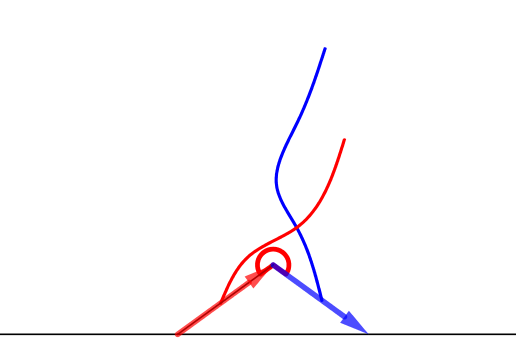
\includegraphics[scale=1]{ILCFig10_non_a_}
			\caption{}
\label{fig:diss(a)}
		\end{subfigure}
		\hfill
		% Subfigure (b)
		\begin{subfigure}{0.45\textwidth}
			\centering
			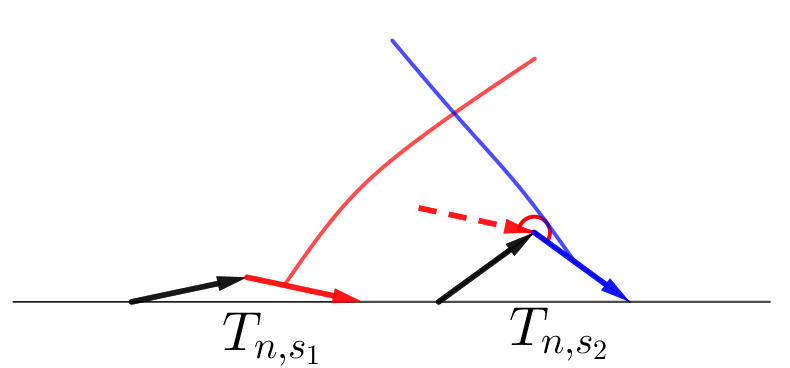
\includegraphics[scale=1]{ILCFig10_non_b_}
			\caption{}
\label{fig:diss(b)}
		\end{subfigure} \\
		
		\begin{subfigure}{0.45\textwidth}
			\centering
			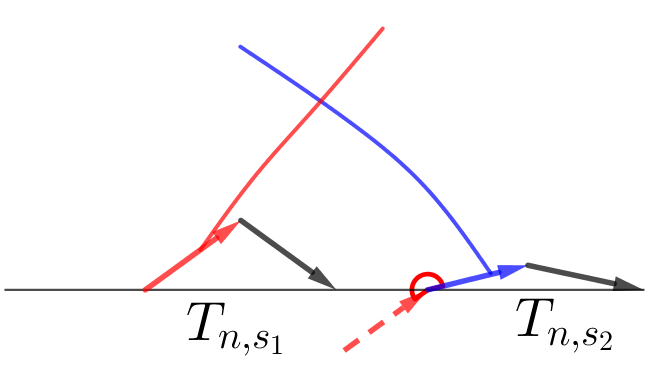
\includegraphics[scale=1]{ILCFig10_non_c_}
			\caption{}
\label{fig:dissrec(c)}
		\end{subfigure}
		\hfill
		% Subfigure (b)
		\begin{subfigure}{0.45\textwidth}
			\centering
			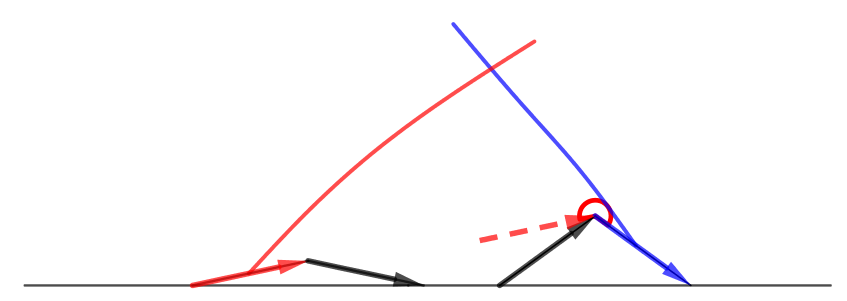
\includegraphics[scale=1]{ILCFig10_non_d_}
			\caption{}
\label{fig:dissrec(d)}
		\end{subfigure}
		\caption{Non-convex crossings scenarios. In case (b), $s_{1}<S_{2}$; whereas in case (c), $s_{1}>s_{2}$.}
		\label{fig:nonconvex}
	\end{figure}


\begin{figure}[H]
			\centering
			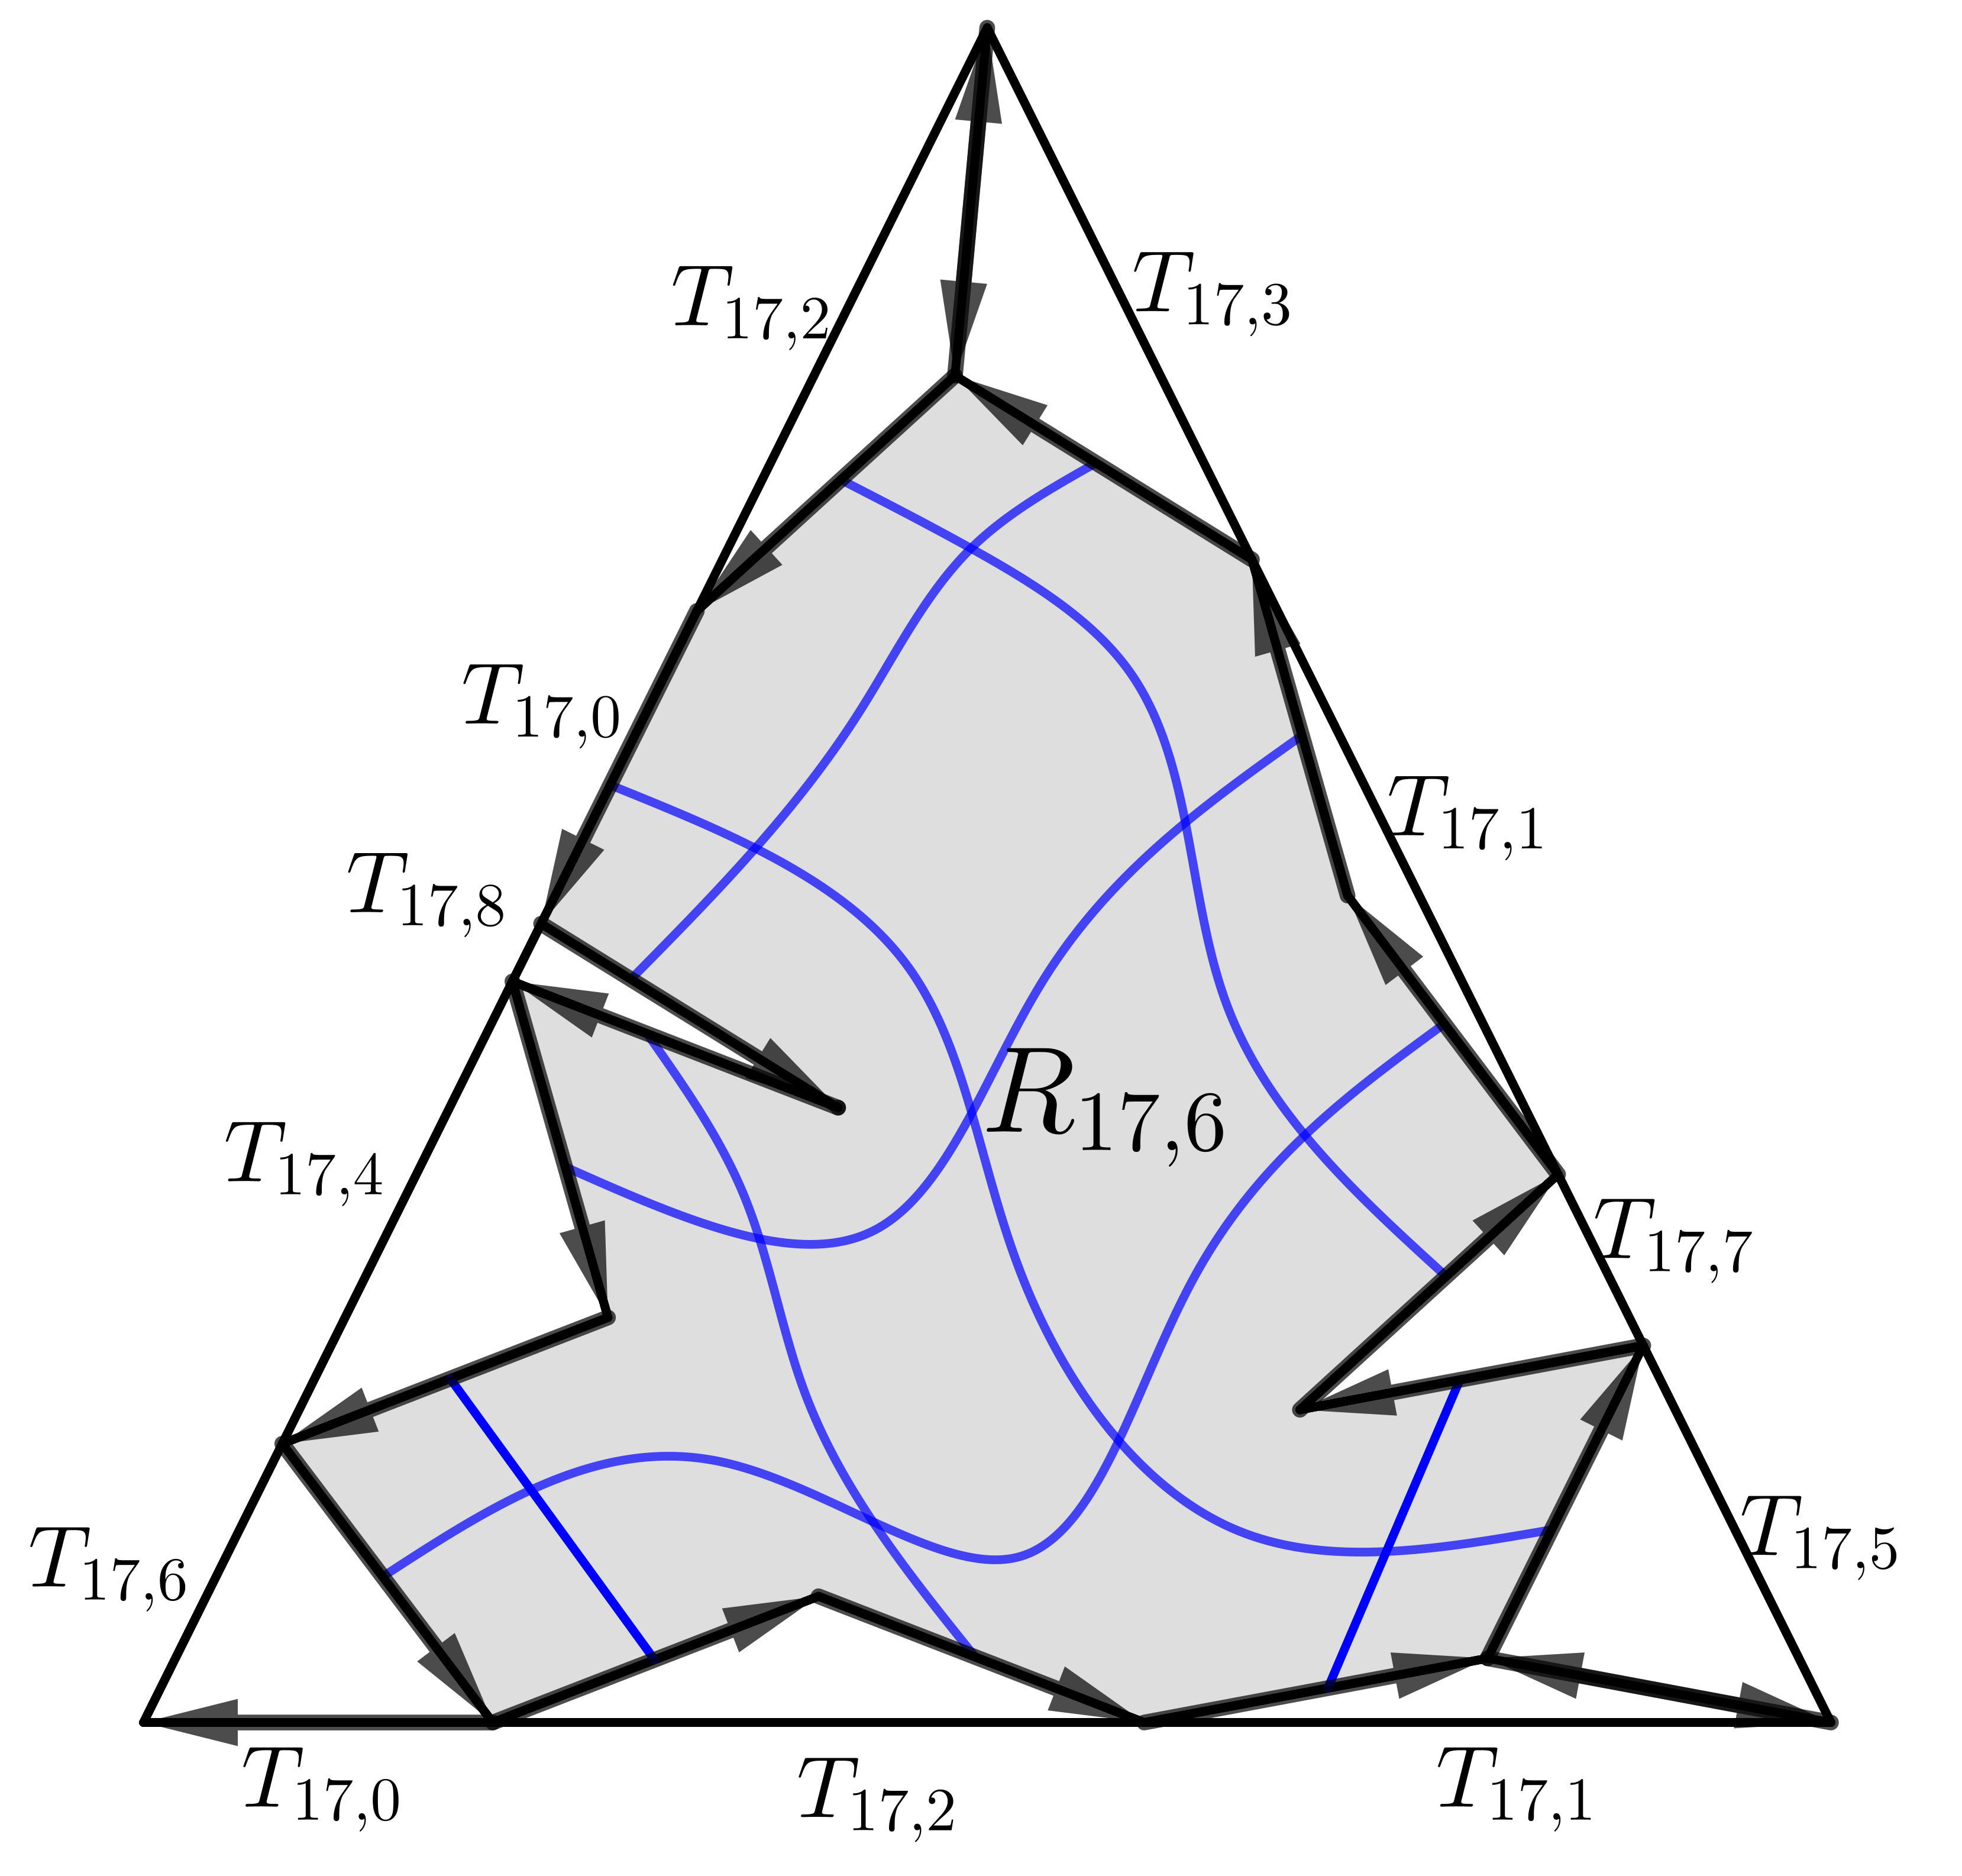
\includegraphics[scale=.11]{ILCFig11_convex}
		\caption{A region $R_{17,6}$ that satisfies the convex crossing.}
		\label{fig:correctdissection}
	\end{figure}


\begin{rem}
For the cases \(k = 1\) and \(k = (n-1)/2\), the total area of the initial tiles is equal to the area of \(\mu_{n} T_{n,k}\). In this situation, matched edges overlap. Since at least one of the interior angles is \(\pi/n\), the tiles are straightforward to arrange once a tile equivalent to \(T_{n,1}\) is placed at the left or right corner of the large triangle for \(k = 1\), or at the apex for \(k = (n-1)/2\). Using the matching of edges determined by the corresponding angles, the placement of the remaining tiles proceeds in a cascading manner, much like a domino effect.
\end{rem}

\begin{rem}
We note that all values of \(n\) and \(k\) satisfy the balance condition, whereas a few values of \(k\) do not satisfy the convex-crossing condition. We have observed that \(R_{n,k}\) is easier to dissect when the number of non-convex crossings is minimized. In fact, even when a non-convex crossing occurs, it is still possible to associate chains of rhombs with the curves forming the non-convex crossing, although these chains are interrupted along a line (see, for example, \(\sigma_{17}(T_{17,5})\) and \(\sigma_{17}(T_{21,3})\)). This observation suggests further study. Based on examples, including some not presented here, we conjecture that a version of the KSK criterion for isosceles triangles can be formulated.
\end{rem}
